
The authors provided us with three graphs in order to test our
different implementations of the Tutte method.\\

These graphs have the following characteristics :

\begin{center}
\begin{tabular}{|c|c|c|}
\hline
Graph & number of vertices & number of edges \\
\hline
aiir\_traffic & 14693 & 63403\\
imdb & 9488 & 33942\\
migration & 14318 & 49460\\
\hline
\end{tabular}
\end{center}


For the first implementation with a basic structure to
work on the graph, we obtain these results~:

\begin{center}
\begin{tabular}{|c|c|c|c|}
\hline
Graph & number of iterations & mean time of execution of Tutte's algorithm & standard deviation\\
\hline
aiir\_traffic & 61 & 0.2526 & 0\\
imdb & 473 & 1.2957 & 0\\
migration & 5 & 0.006314 & 0\\
\hline

\end{tabular}
%\caption{title}
\end{center}

The results we get here is not as good as we expected. Although the
computation time is quite improved, the produced graph is not planar.  The
reason is because the graph provided has some fixed nodes inside the
grid. Consequently, after the call of our implementation of the Tutte
Algorithm, some edges crossing (due to those fixed nodes) appear and remove
the planarity of the graph.

As an explanation, we can say that by moving nodes around an internal fixed
node, and in relation with the number of edges in one side of the graph, mobile
nodes tend to orient themselves to the side of the fixed node having
most of edges (see the figure \ref{mauvais_1}). With a such graph, a
mobile node which is opposite to the side with a lot of edges will move to
this side and create an edge-crossing (see the figure \ref{mauvais_2}).

Here are some pictures:

% \begin{figure}[!h]
% \centering
% 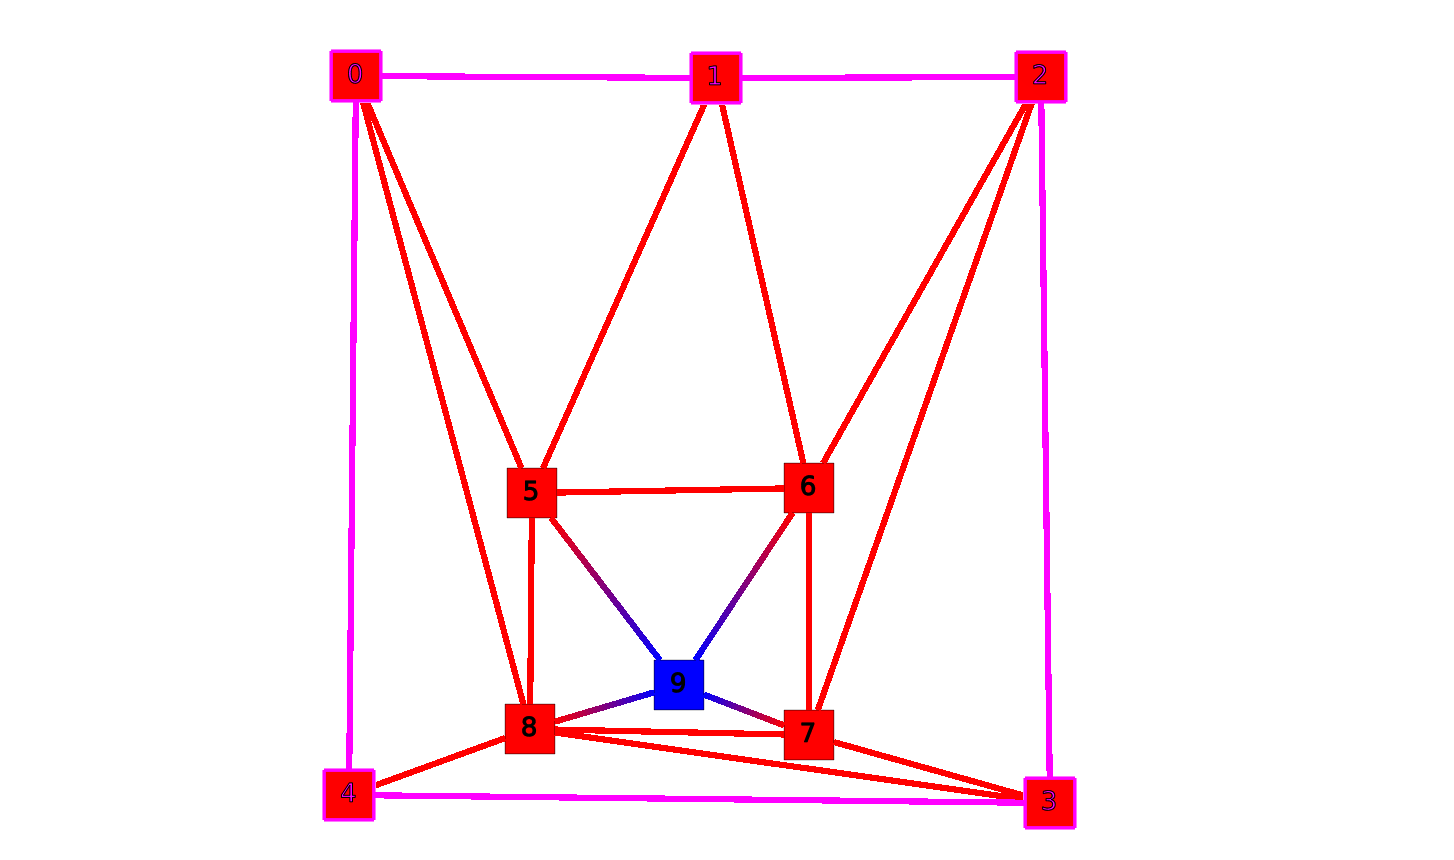
\includegraphics[scale=0.25]{snapshots/constate_fix_init.png}
% \caption{One initial set}
% \label{mauvais_1}
% \end{figure}

% \begin{figure}[!h]
% \centering
% 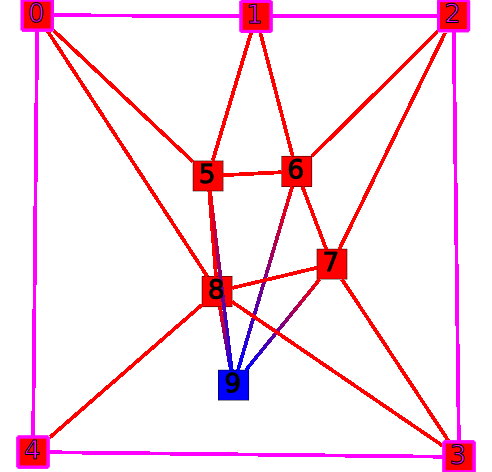
\includegraphics[scale=0.25]{snapshots/constate_probleme.png}
% \caption{The set not correctly modified(one fixed node)}
% \label{mauvais_2}
% \end{figure}


\begin{figure}[!h]
  %\begin{minipage}[!h]{.46\linewidth}
  \begin{minipage}[!h]{.5\linewidth}
   \centering
   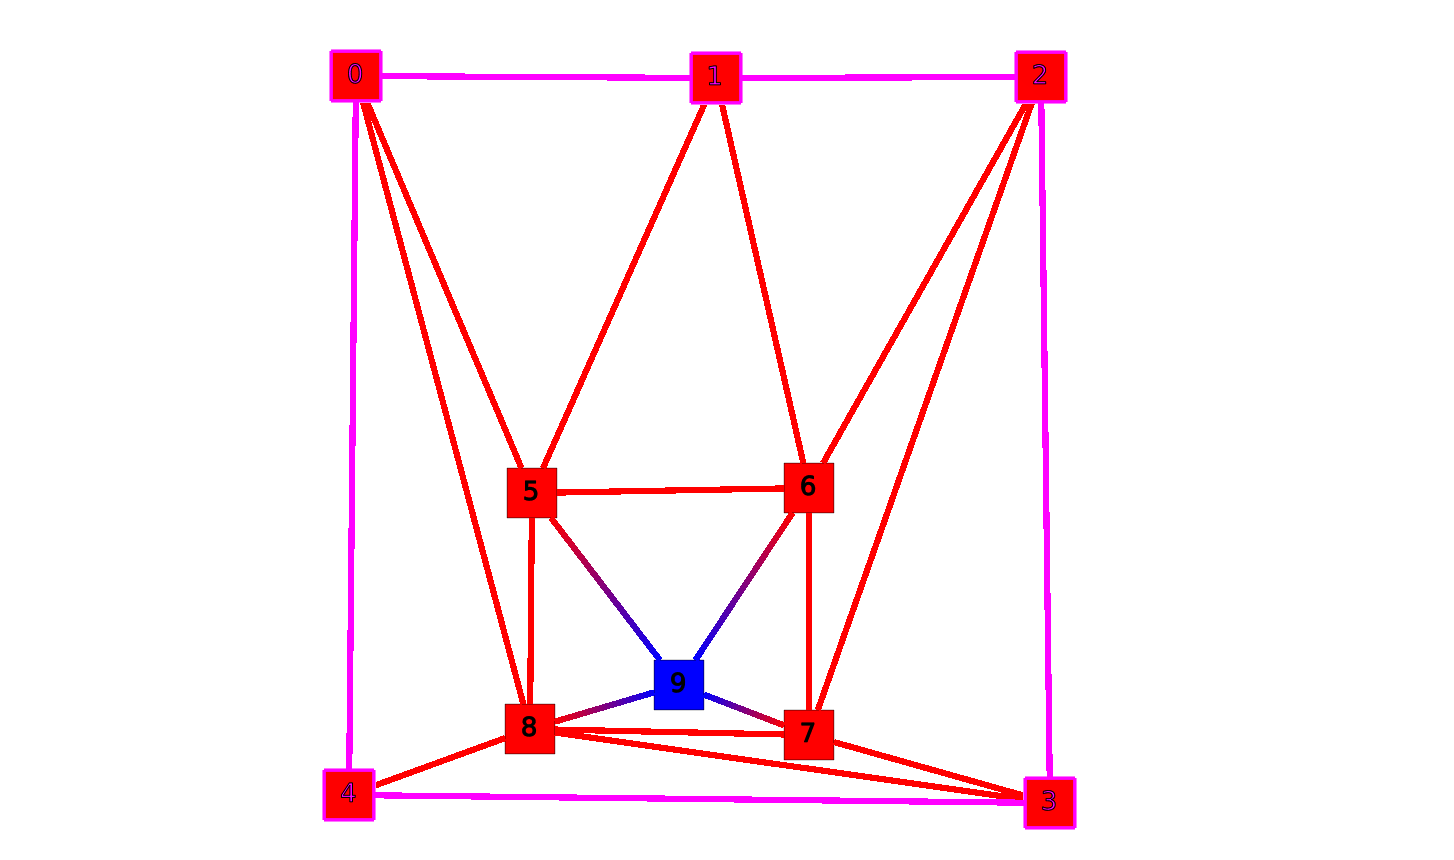
\includegraphics[scale=0.25]{snapshots/constate_fix_init.png}
   \caption{One initial set}
   \label{mauvais_1}
 \end{minipage} \hfill
 \begin{minipage}[!h]{.3\linewidth}
   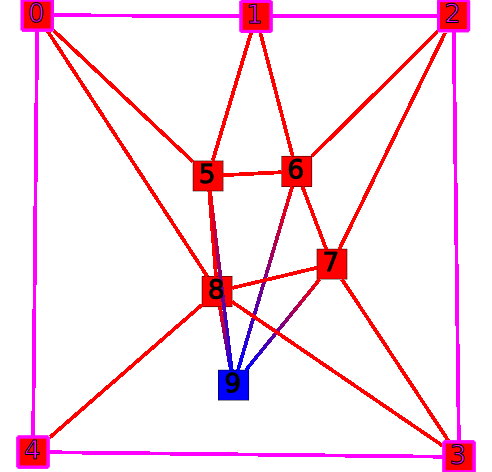
\includegraphics[scale=0.35]{snapshots/constate_probleme.png}
   \caption{The set not correctly modified(one fixed node)}
   \label{mauvais_2}
 \end{minipage}
\end{figure}

\begin{figure}[!h]
\centering
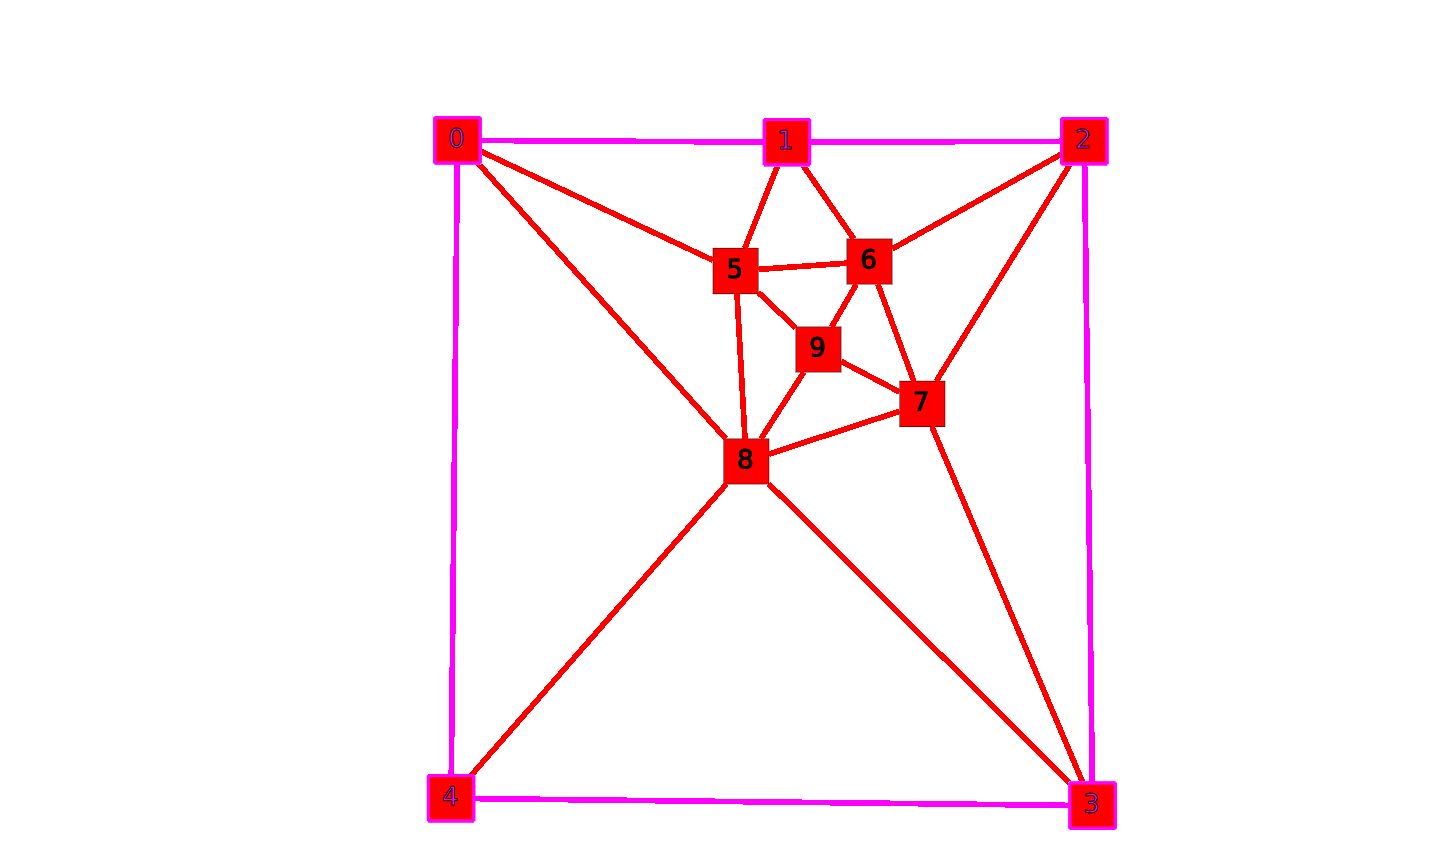
\includegraphics[scale=0.25]{snapshots/constate_nikel.png}
\caption{The set correctly modified(all nodes mobiles)}
\end{figure}

